\section{Introduction}
\label{sec:introduction}

% state the learning objective
\par The objective of this laboratory assignment is to study two methods for circuit analysis: the mesh method and the nodal method. The circuit to be analysed is composed of resistors and dependent and independent voltage and current sources. The circuit can be seen if Figure~\ref{fig:rc}. 

\par In Section~\ref{sec:analysis}, a theoretical analysis of the circuit is presented, showing the derived equation systems and respectively calculated voltage and current values. The circuit only contains passive elements and the independent sources produce constant outputs, therefore the solution of the circuit is stationary and the results will be presented as constant values.
\par In Section~\ref{sec:simulation}, the circuit is analysed by
simulation, using the software NGSpice, and the results are compared to the theoretical results obtained in
Section~\ref{sec:analysis}. The conclusions of this study are outlined in
Section~\ref{sec:conclusion}.

\begin{figure}[H]
\centering
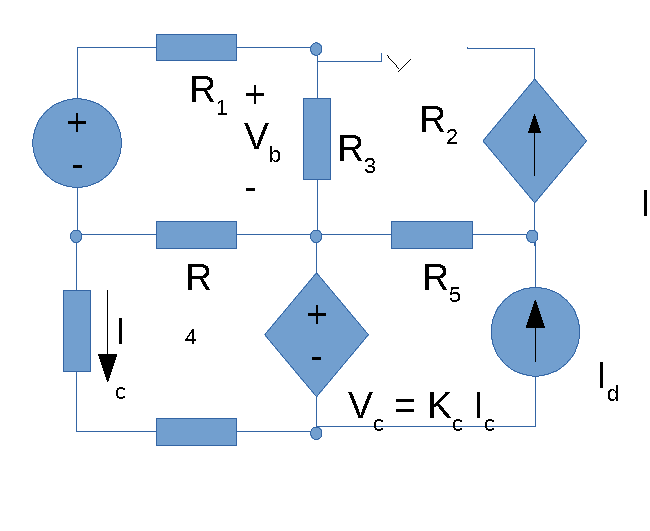
\includegraphics[width=10 cm]{rc.pdf}
\caption{Voltage driven serial RC circuit.}
\label{fig:rc}
\end{figure}
